\documentclass[../notesdecours.tex]{subfiles}

\begin{document}

\chapter{Applications des postulats de la Mécanique Quantique}

\section{Interféromètre de Mech-Zehnder}
Cet exemple est tiré de l'optique. Nous allons regarder ce qu'il se passe en optique classique, et nous allons ensuite utiliser le formalisme quantique. Ce faisant, nous pourrons mettre en évidence les différences entre les deux. \\

\begin{center}
    \begin{figure}[h]
    \centering
    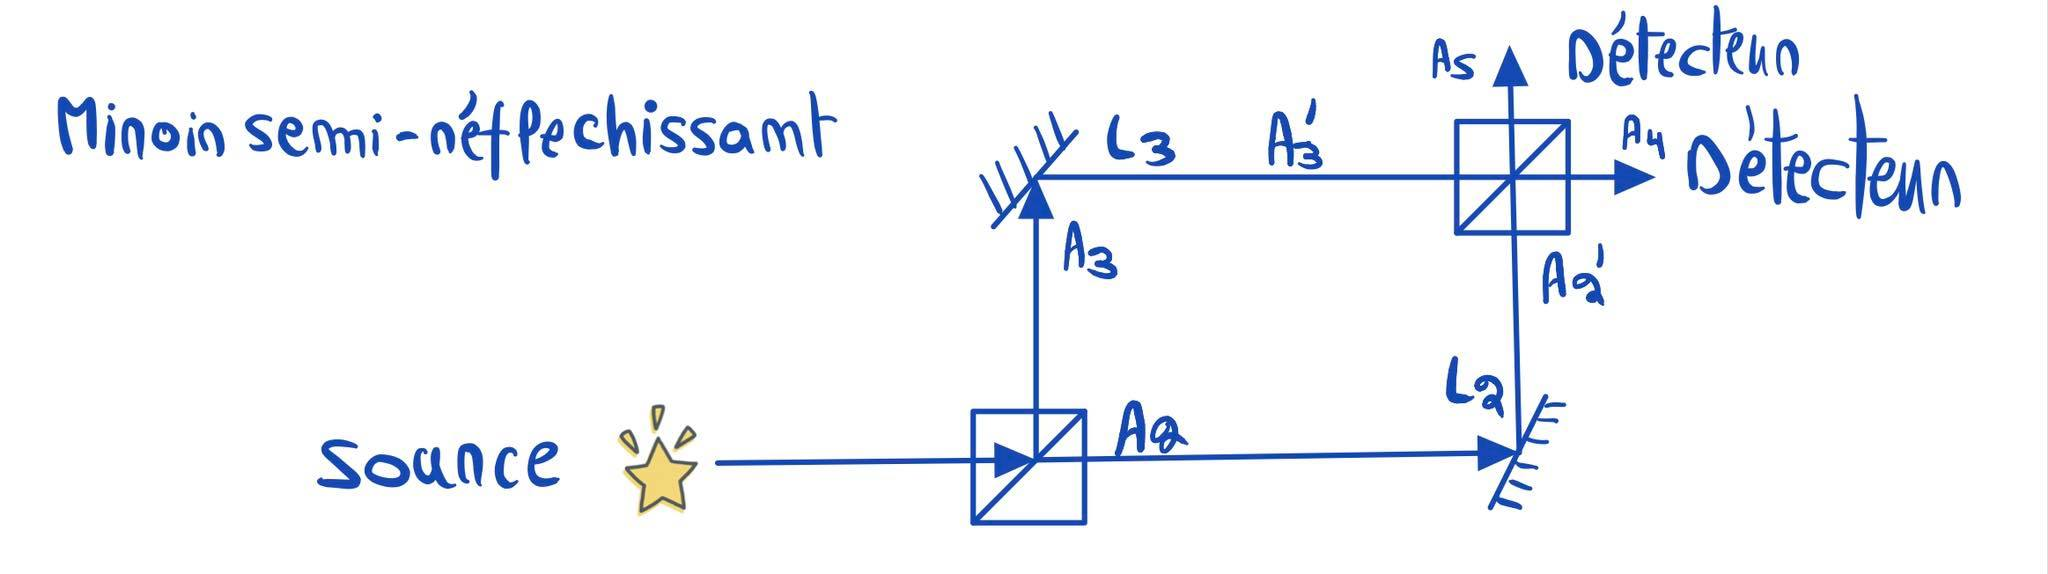
\includegraphics[width=0.80\textwidth]{Mach-Zehnder.png}
    \caption{Représentation du principe de l'interféromètre de Mach-Zehnder. Notons que les longueurs $L_i$ représentent la longueur totale du trajet dans le chemin $i$ suivit.}
    \label{Mach-Zehnder}
    \end{figure}
\end{center}

\subsection{Brève description des détecteurs}
Au niveau des détecteurs, plusieurs chemins sont possibles, comme l'illustre l'image ci-contre.

\begin{center}
    \begin{figure}[h]
    \centering
    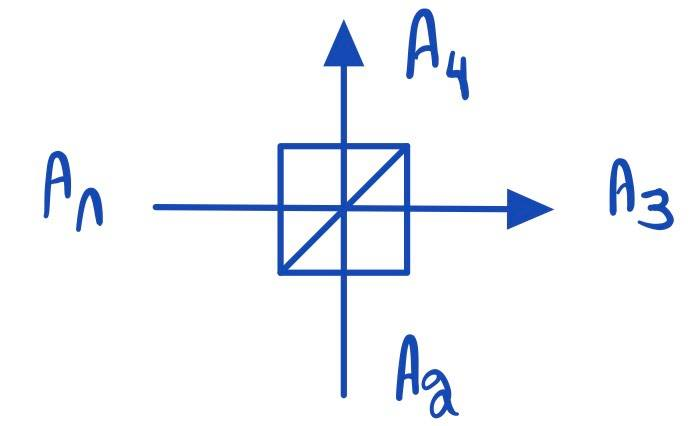
\includegraphics[width=0.50\textwidth]{bean.png}
    \caption{Les ondes incidentes arrivants de $A_1$ et $A_2$ poursuivent leur chemin, respectivement en $A_3$ et $A_4$.}
    \label{Interferometre}
    \end{figure}
\end{center}

Nous avons un miroir semi-transparant. Nous envoyons dessus par le port 1 un faiseau de lumière d'amplitude $A_1$, et d'intensité $I_1 = \norm{A_1}^2$ ; par le port 2, nous envoyons un faisceau d'amplitude $A_2$ et d'intensité $I_2 = \norm{A_2}^2$. \emph{En supposant qu'il n'y a pas de pertes}, nous avons que la somme des intensités entrantes est égale à la somme des intensités sortantes : $I_1 + I_2 = I_3 + I_4$. Puisque les équations de l'électromagnétisme sont linéaires, nous avons $A_3 = \alpha A_1 + \beta A_2$, pour tout $\alpha,\beta\in\mathbb{C}$. Nous pouvons facilement mesurer les valeurs absolues de ces coefficients. En posant $A_2 = 0$, nous pouvons mesurer $I_3$ ; nous trouverons $\norm{\alpha}^2$.

Partons de la description d'une onde plane. Nous aurons
\begin{subequations}
    \begin{equation}
        A_1 (t) = A_1e^{-i\omega t},
    \end{equation}
    \begin{equation}
        A_2 (t) = A_2e^{-i\omega t},
    \end{equation}
\end{subequations}

pour les ondes incidentes, ainsi que
\begin{subequations}
    \begin{equation}
        A_3 (t) = cA_1e^{-i\omega t} + i s A_2e^{-i\omega t}
    \end{equation}
    \begin{equation}
        A_4 (t) = c A_2e^{-i\omega t} + i sA_1e^{-i\omega t}
    \end{equation}
\end{subequations}

pour les ondes sortantes. La discussion précédente nous permet de choisir un des coefficients - soit $\norm{c}^2$ - en choissisant le miroir semi-transparent. Le coefficient $\norm{s}^2$ est alors fixé par

\begin{equation}
\norm{c}^2 + \norm{s}^2 = 1.
\end{equation}

Il nous reste une liberté de phase : nous pouvons redéfinir la phase de $A_1 = e^{i \Phi}A'_1$, et de même pour $A_2, A_3$ et $A_4$. Il s'agit d'une question de convention.

\begin{remark} 
    Par convention, les ondes transmises ne subissent aucun déphasage, là où les ondes réfléchies bénéficient d'un déphasage de $\frac{\pi}{2}$. D'autres conventions sont possibles.
\end{remark}

\begin{remark} 
    Nous pouvons prendre $c = \cos\theta$ et $s = \sin\theta$ pour un argument $\theta$, ce qui explique la notation utilisée. 
\end{remark}

\subsection{Lumière classique}
Pour simplifier, prenons $c = \frac{1}{\sqrt{2}} = s$. Notons que nous pouvons introduire un facteur $e^{ikL}$ tenant compte de la distance parcourue, i.e. un point en $x = 0$ peut-être décrit par $A(t) = Ae^{-i\omega t}$ et un point en $x = L$ peut-être décrit par $A'(t) = Ae^{-i\omega t}e^{ikL}$. Notre détecteur repère le courant électrique $I(t)$ selon $I(t) = e\norm{A(t)}^2$ - soit 

\begin{align*}
A(t) &= Ae^{-i\omega t}	&I_{0} = \norm{A(t_0 = 0)}^2 = \norm{A}^2.
\end{align*}

Nous avons alors que

\begin{align*}
A_2 (t) &= \frac{A(t)}{\sqrt{2}}	&A_3 (t) = i\frac{A(t)}{\sqrt{2}}
\end{align*}

En particulier, nous pouvons écrire les chemins $A_2'$ et $A_3'$ selon:
\begin{subequations}
    \begin{align}
        A'_2 (t) &= A_2 (t)e^{ikL_2}	&A'_3 (t) = A_3 (t)e^{ikL_3}
    \end{align}
\text{De même, les chemins $A_4$ et $A_5$ s'écrivent:}
    \begin{align}
        A_4 &= \frac{1}{\sqrt{2}} (A'_3 + iA'_2) = i\frac{A(t)}{2} (e^{ikL_3} + e^{ikL_2})		&A_5 = \frac{A(t)}{2} (e^{ikL_2} - e^{ikL_3})  
    \end{align}
\end{subequations}

En introduisant le terme $\Delta \Phi = kL_3 - kL_2$, nous pouvons conclure que:
\begin{subequations}
    \begin{align}
        I_4 &= \frac{\norm{A}^2}{4} \norm{e^{ikL_2} + e^{ikL_3}}^2 = \norm{A}^2 \cos^2 \frac{k(L_3-L_2}{2} = \norm{A}^2 \cos^2 \frac{\Delta\Phi}{2}\\
        I_5 &= \norm{A}^2 \sin^2 \frac{\Delta \Phi}{2}
    \end{align}
\end{subequations}

Remarquons que $I_4+I_5 \doteq I_{0}$ - soit $I_0 = \norm{A}^2$, comme prévu. Hourra.

\subsection{Lumière quantique}

Le photon peut suivre plusieurs chemin simultanément : par superposition, nous écrivons l'état comme

\begin{equation}
    \ket{\psi} = \alpha\ket{1}+\beta\ket{2}+\gamma\ket{3}
\end{equation}
Où $\ket{i}$ décrit le photon dans le chemin $i$.\\

Dans un beam splitter tel que décrit par \eqref{Interferometre}, nous décrivons alors les transitions
\begin{align}
    \ket{1} &\rightarrow c\ket{3} + is\ket{4},\\
    \ket{2} &\rightarrow is\ket{3} + c\ket{4}.
\end{align}
Cette transition est décrite par la matrice  $\begin{pmatrix}
c & is\\
is & c
\end{pmatrix}$, unitaire.\\

Soit une mesure dans la base $\ket{1},\ket{2}$ ; donnée par l'était $\ket{\psi} = \alpha\ket{1}+\beta\ket{2}$. Dès lors, les probabilités de détection seront données par $P_1 = \norm{\alpha}^2$ et $P_2 = \norm{\beta}^2$.\\

Il s'ensuit que la decription de l'interféromètre \ref{Interferometre} sera la suivante:

\begin{itemize}
    \item \textbf{Chemins 2 et 3.}
        \begin{equation}
            \ket{\psi} = \frac{1}{\sqrt{2}}\ket{2} + \frac{1}{\sqrt{2}}\ket{3}
        \end{equation}
    \item \textbf{Chemins 2' et 3'.}
        \begin{align}
            \ket{\psi} &= \frac{e^{ikL_2}}{\sqrt{2}}\ket{2'} + \frac{i}{\sqrt{2}}e^{ikL_3}\ket{3'}\\
        \end{align}
    \item \textbf{Chemins 4 et 5.}
        \begin{align}
            \ket{\psi} &= \frac{1}{2} (e^{ikL_2} - e^{ikL_3})\ket{5} + \frac{i}{2}(e^{ikL_2} + e^{ikL_3})\ket{4}
        \end{align}
\end{itemize}

Dès lors,nous avons que les probabilités de détections en 4 et en 5 seront:
\begin{align}
    P_4 &= \cos^2 \frac{\Delta \Phi}{2}\\
    P_5 &= \sin^2 \frac{\Delta \Phi}{2}
\end{align}
\emph{Le photon est simultanément dans les chemins 2 et 3.}\\

Remarquons que si nous supprimons le beam splitter à la fin, les probabilités de présence se réduisent à
\begin{equation}
    P_4 = \frac{1}{2} = P_5
\end{equation}

Les \emph{delayed choice experiment} (Wheeler, 1978) - qui consistent à enlever/remettre le beam splitter, ou à changer la phase $\Delta\Phi$ après que le photon soit entré dans l'interféromètre - nous apprennent que \textbf{toute interprétation ou l'on suppose que le photon "sait à l'avance ce qu'il doit faire", ne tient pas.}

% \section{Oscillations de neutrinos}
% Les neutrinons sont des particules neutres, intéragissant très faiblement avec la matière. Elle fût prédite par Pauli pour expliquer le spectre des $e^-$ dans la désintégration du $\beta : n \Rightarrow p^+ + e^- + \nu$.

% \section{MASER $NH_3$}
% Dans cette section, nous allons discuter d'un appareil fort pratique: le MASER\footnote{Acronyme anglais pour 'Microwave Amplicifaction by Stimulated Emission of Radiation'.} d'ammonium $NH_3$ ; l'un des ancêtres des LASER\footnote{Acronyme anglais pour 'Light Amplification by Stimulated Emission of Radiation'.}

\section{Résonance quantique}

\subsection{Exemple 1 : l'atome de $NH_3$}

\color{red} \textbf{Insérer graphique.} \color{black}

Dans la base $\{\ket{1},\ket{2}\}$, l'Hamiltonien de ce système s'exprime par
\begin{equation}
    H = 
    \begin{pmatrix}
        E_0 & -A\\
        -A & E_0
    \end{pmatrix}
\end{equation}
Il se trouve que dans la base $D = \{\ket{E_0-A},\ket{E_0+A}\}$ des états propres d'énergie, cette matrice est diagonale. Nous observons alors que l'énergie fondamentale $E_0 > E_0-A$. Nous en concluons que si l'atome peut effectivement être stable dans l'état non-dégénéré d'énergie $E_0$, il l'est encore plus dans l'état doublement dégénéré d'énergie $E_0-A$. D'autres exemples similaire existent, tel que celui de la molécule de Benzène.

% \subsection{Ion moléculaire $H_2^+$}

% Bla,bla, ... compléter !

\section{Spin $\frac{1}{2}$ : quantification du moment angulaire}
Nous présentons dans cette section une autre application des postulats de la Mécanique Quantique évoqués au chapitre précédent. L'expérience de Stern-Gerlach a permis de mettre en avant une \textbf{quantification du moment angulaire} observée expérimentalement. Cet effet purement quantique sera brièvement étudié dans cette section (plutôt "introduit" ici, et étudié dans le cours de BA3). Nous allons utiliser les postulats de la Mécanique Quantique pour formaliser la quantification du moment angulaire. \\

\begin{leftbar}
    \textit{Une particule de spin $1/2$ est une particule dont la composante du moment cinétique dans une direction (disons $O_z$) peut prendre les valeurs $-1/2$ ou $1/2$. }
\end{leftbar}

Plus précisément, étant donné que nous parlons d'une grandeur physique, nous allons voir quelle observable la représente, et que ce sont les propriétés de cette observable qui impliqueront la \textbf{quantification} de ses valeurs propres. Nous allons également étudier la \textbf{conservation} du moment cinétique voir que cet effet est dû à un principe très cher en physique : l'\textbf{invariance par rotation}. \\

Dans cette section, l'étude du moment cinétique est organisé en trois parties :
\begin{enumerate}
    \item Le lien avec les rotations : introduction au groupe des rotations ;
    \item L'invariance par rotation et la quantification du moment angulaire ;
    \item Application : représentation du groupe des rotations en 2D par les matrices de Pauli, et mise en avant des vecteurs propres.
\end{enumerate} 

\paragraph{Remarque sur les moments cinétiques en mécanique quantique}
Nous commencerons cette section en discutant de l'équivalent quantique du moment cinétique classique $\mathcal{\mathbf{L}}$, et nous enchaînerons ensuite sur une description générale du moment cinétique \textbf{total} d'une particule en mécanique quantique, qu'on note $\mathbf{J}$, composé :
\begin{itemize}
    \item du moment cinétique angulaire (aussi appelé "moment cinétique orbital") $\mathbf{L}$, dû au mouvement de la particule (par exemple, dans un potentiel central comme en mécanique classique) ;
    \item et du moment cinétique intrinsèque (ou "moment cinétique de spin"), noté $\mathbf{S}$, celui intervenant dans l'expérience de Stern-Gerlach et n'ayant aucun équivalent classique.
\end{itemize}


\subsection{Groupe des rotations}

Le titre de cette section mène à la définition des deux notions suivantes :
\begin{definition}
    Un groupe $G$ est un ensemble d'élements, muni d'une opération ("opération de groupe", ou "loi de composition") notée "$\cdot$" qui satisfait les propriétés suivantes :
    \begin{itemize}
        \item Le produit est interne : $\forall g_1, g_2 \in G : g_1\cdot g_2 \in G$
        \item Le produit est associatif : $\forall g_1, g_2, g_3 \in G : g_1\cdot(g_2\cdot g_3) = (g_1\cdot g_2)\cdot g_3.$
        \item Existence d'un élément neutre : $\exists e\in G \; \text{t.q} \; \forall g \in G \; : \; e\cdot g = g = g\cdot e$.
        \item Existence d'un inverse pour tout élément du groupe : $\forall g \in G\; ,\; \exists g^{-1}\in G \; \text{t.q} \; g^{-1}\cdot g = e = g\cdot g^{-1}.$
    \end{itemize}
\end{definition}
\begin{definition}(Issue du Cohen-Tannoudji, ch. VI)
    Une rotation géométrique est une \textbf{transformation} dans l'espace tridimensionnel qui conserve un point, les angles, les distances ainsi que le sens des trièdres\footnote{Pour exclure les symétries du plan}.
\end{definition}


Les rotations sont d'une importance particulière en physique, car de nombreux objets, pas seulement les vecteurs de l'espace tridimensionnel, se transforment sous l'action d'une rotation. Ainsi, nous généralisons la notion de rotation à l'appartenance à un groupe, le \textbf{groupe des rotations}. \\

Le groupe des rotations, noté $SO(3)$ sera amplement étudié dans les cours de maths, et de mécanique quantique de BA3, mais nous pouvons intuitivement accepter que les rotations constituent en effet un groupe, de par leur loi de composition interne et associative, l'existence d'un neutre (la rotation identité) et d'une rotation inverse. \\

Pour le formaliser, il reste à insister sur la conservation de la norme. Ainsi, les rotations seront généralisées à des "éléments du groupe des rotations", et les éléments de ce groupe pourront être représentés par des matrices \textbf{orthogonales}. Prenons le cas classique et nous obtenons des matrices orthogonales $3\times 3$.

$$R\in \mathbb{R}^{3\times3} \quad |\quad R^T R = \mathbb{I}$$

Une rotation est paramétrée par 
\begin{itemize}
    \item $\vec n$, l'axe de rotation (vecteur unitaire);
    \item $\theta$, l'angle de rotation.
\end{itemize}
On note $R(\theta, \vec n)$ la rotation (dans le sens antihorlogique) autour de l'axe $\vec n$, d'un angle $\theta$. Dans l'espace tridimensionnel, $\vec{n} \in \mathbb{R}^3$, et nous avons les matrices suivantes, bien connues, implémentant les rotations autour des trois axes usuels. Elles peuvent être notées d'une autre manière, introduisant les matrices $L_x, L_y, L_z$ (qui auront une importance particulière par la suite).

$$
\begin{array}{llr}
    R(\theta, \vec{1}_x) = 
    \left(
        \begin{array}{ccc}
            1&0&0 \\
            0&\cos\theta& -\sin\theta\\
            0&\sin\theta& \cos\theta\\
        \end{array}
    \right) & =\exp(i\theta L_x), 
        &L_x = \left(
            \begin{array}{ccc}
                0&0&0 \\
                0&0&i \\
                0&-i&0
            \end{array}
        \right)
    \\
    \vspace{1cm} \\
    R(\theta, \vec{1}_y) = 
    \left(
        \begin{array}{ccc}
            \cos\theta & 0 & \sin\theta \\
            0&1&0 \\
            -\sin\theta & 0 & \cos\theta \\
        \end{array}
    \right) &=\exp(i\theta L_y),
        &L_y = \left(
            \begin{array}{ccc}
                0&0&-i \\
                0&0&0 \\
                i&0&0
            \end{array}
        \right)
    \\
    \vspace{1cm} \\
    R(\theta, \vec{1}_z) = 
    \left(
        \begin{array}{ccc}
            \cos\theta & -\sin\theta & 0 \\
            \sin\theta & \cos\theta & 0 \\
            0&0&1 \\
        \end{array}
    \right) &=\exp(i\theta L_z),
        &L_z = \left(
            \begin{array}{ccc}
                0&i&0 \\
                -i&0&0 \\
                0&0&0
            \end{array}
        \right)
\end{array}
$$

D'une manière générale, nous pouvons écrire
\begin{align}
    R(\theta, \vec n) &= \exp(i\theta \vec n \cdot \vec L) && \text{où} \; \vec n \cdot \vec L = n_xL_x + n_yL_y + n_zL_z \; . \\
    &= \mathbb{I} + i\theta \vec{n} \cdot \vec L + O(\theta^2) \label{eq:ch5-spin-generateurs}
\end{align}

L'introduction de ces opérateurs $L_i$ est très intéressante car en théorie des groupes, lorsque nous pouvons écrire \ref{eq:ch5-spin-generateurs}, nous disons que les opérateurs $L_x, L_y, L_z$ sont les \textbf{générateurs du groupe des rotations}. L'interprétation en est facile : prenons par exemple une rotation autour de l'axe $\vec 1_x$ d'un angle infinitésimal $\mathrm{d}\theta$.
$$R(\mathrm{d}\theta, \vec 1_x) = \mathbb{I} + iL_x \; \mathrm{d}\theta \qquad \text{au premier ordre}$$

La rotation diffère de l'opérateur identité d'un facteur $\mathrm{d}\theta$ au coefficient $L_x$ au premier ordre. $L_x$ est alors dit un "générateur infinitésimal", et en théorie des groupes, dans un groupe de Lie \footnote{Voir définition dans le cours de maths}, l'étude des générateurs infinitésimaux suffit à reconstruire tout le groupe. 

\subsubsection{Relations de commutation du groupe des rotations : algèbre du groupe}
Les relations de commutation sont centrales dans tout groupe. Ici, avec les générateurs que nous avons introduits, nous pouvons mettre en avant les relations de commutation suivantes :
$$
\begin{array}{ll}
    \left[ L_x, L_y \right] &= iL_z \\
    \left[ L_z, L_x \right] &= iL_y \\
    \left[ L_y, L_z \right] &= iL_x \\
\end{array} \; ,
$$
ou, de manière abrégée :
\begin{equation}\label{eq:chap5-spin-commutation}
    \boxed{\left[ L_i, L_j \right] = i\varepsilon_{ijk} L_k} \; .
\end{equation}
Les relations de commutation \ref{eq:chap5-spin-commutation} définissent l'\textbf{algèbre de Lie} du groupe $SO(3)$\footnote{Ou de manière équivalente, l'algèbre de commutation des générateurs infinitésimaux du groupe.}.
\paragraph{Interprétation des relations de commutation}

{\color{red}{je ne réussis pas à obtenir les mêmes termes, et je ne comprends pas l'interprétation. J'ai trouvé un équivalent  en mécanique classique dans le Cohen-Tannoudji.}}
$$
\begin{array}{llr}
    R(-\theta, y)R(-\theta, x)R(\theta, y)R(\theta, x) &= \mathbb{I} + \theta^2\left[L_x, L_y\right] + O(\theta^3)& \\
    &= R(\theta^2, L_z) & \text{à l'ordre} \; \theta^2
\end{array}
$$


\subsection{Représentations du groupe des rotations}
Nous avons vu à la section précédente l'action d'une rotation sur l'espace euclidien tridimensionnel. Seulement, comme déjà mentionné, en physique, les vecteurs ne sont pas les seuls objets pouvant se transformer par une rotation : c'est ce qui motive l'utilisation du groupe des rotations en général plutôt que les matrices $R\in \mathbb{R}^{3\times 3}$ qui représentent les rotations dans l'espace. \\

Ainsi, de manière générale, le groupe des rotations aura plusieurs représentations, l'important étant de retrouver les relations de commutation \ref{eq:chap5-spin-commutation}.

\begin{definition}
    Une représentation de l'algèbre de Lie du groupe des rotations est un ensemble de matrices $J_i$, de taille $n\times n$ a priori arbitraire, satisfaisant les relations de commutation $$ [J_i, J_j] = i\varepsilon_{ijk} J_k$$
\end{definition}

En mécanique quantique, une représentation de $SO(3)$ permet d'implémenter les transformations de rotation de la manière suivante :
\begin{equation} \label{eq:chap5-spin-transformation}
    \ket \psi \stackrel{R(\theta,\vec n)}{\longrightarrow} \exp(i\theta \; \vec n \cdot \vec J) \ket \psi
\end{equation}

Un exemple de représentation est l'équivalent quantique du moment angulaire $\mathbf L= \mathbf{R} \times \mathbf{P}$ (en reprenant la notation $\vec J$):
$$
\begin{array}{ll}
    J_x &= yP_z - zP_y \\
    J_y &= zP_x - xP_z \\
    J_z &= xP_y - yP_x
\end{array}
$$

\begin{leftbar}
    \textit{Cette section a servi à introduire le \textbf{groupe des rotations} : la notion de groupe, de générateur, de représentation. Grâce à cela, nous aboutissons à une définition très générale des opérateurs qui implémentent une transformation de rotation.} \\

    A présent, nous allons utiliser le formalisme introduit, principalement les relations de commutation, pour étudier davantage les rotations en mécanique quantique.
\end{leftbar}
\subsection{Invariance par rotation}
Un système physique $S$ est par définition \textbf{invariant par rotation} si en lui appliquant à un moment donné une rotation quelconque $\mathcal{R}$ et que nous appliquons la même rotation à tous les systèmes ou appareils qui peuvent influer sur lui, ses propriétés et son comportement ne sont pas modifiés. \\

En particulier, l'invariance par rotation en mécanique quantique veut dire entre autres que l'évolution d'un système se déroule de la même manière que s'il avait préalablement été sujet à une rotation. En pratique :
\begin{itemize}
    \item L'évolution dans le temps est décrite par l'équation de Schrödinger, et indique que $\ket{\psi(t)} = e^{-it \; H}$
    \item Une rotation est générée par le moment cinétique du système, $\vec J$ (voir \eqref{eq:chap5-spin-transformation} pour l'implémentation de cette transformation)
\end{itemize}

Ainsi, en mécanique quantique, un système est invariant par rotation si 
$$
\underbrace{e^{-it\; H}}_{\text{Evol. temps}} \; 
\underbrace{e^{i\theta \; \vec n\cdot \vec J}}_{\text{Rotation}} \; 
\ket \psi = 
e^{i\theta \; \vec n\cdot \vec J}\; 
e^{-it\; H} \; 
 \ket \psi 
 \qquad \forall\;  \ket \psi , \vec n, \theta, t
$$
Et cette condition doit être vraie pour tout $\theta$ et $t$, que l'on peut peut prendre arbitrairement petits, pour obtenir la condition 

\begin{equation}
    [H, J_x] = [H, J_y] = [H, J_z] = 0
\end{equation}
{\color{red}{Je ne suis pas sûr du calcul qui mène à cela. J'arrive à $[H, J_x] + [H, J_y] + [H, J_z] =0$ et je ne vois pas comment affirmer la condition ci-dessus}}

Qui correspond à une traduction de l'invariance par rotation : il faut et suffit que $H$ commute avec les opérateurs de rotations infinitésimales, qui correspondent aux trois composantes du moment cinétique total $\vec J$ du système.

\subsubsection{Conséquences de l'invariance par rotation}
L'invariance par rotation implique la \textbf{conservation du moment angulaire}. Montrons-le en deux temps :
\begin{enumerate}
    \item Si $\ket{\psi(t)}$ est solution de l'équation de Schrödinger $i\partial_t \ket\psi = H\ket\psi$, alors 
    $$\begin{array}{ll}
        \bra{\psi(t)}J_x\ket{\psi(t)} &= \bra{\psi(0)} e^{it\; H} J_x e^{-it\; H}\ket{\psi(0)} \\
        \strut \\
        &= \bra{\psi(0)}J_x\ket{\psi(0)} \; ,
    \end{array}$$ 
    étant donné que $J_x$ et $e^{\pm it\; H}$ commutent (vu que $H$ et $J_x$ commutent) {\color{red}{je ne suis pas sûr de cette justification}}. La relation que nous venons d'obtenir montre que si $J_x$ est une observable, \textbf{sa valeur moyenne dans l'état $\psi$ est constante à travers le temps}.

    \item Si $\ket \psi$ est vecteur propre de $J_x$ :
    $$J_x\ket \psi = j \ket \psi$$
    Alors, $\ket{\psi(t)} = \exp(-it\; H)\ket\psi$ est aussi un vecteur propre de $J_x$, avec la même valeur propre :
    $$
    \begin{array}{ll}
        J_x \ket{\psi(t)} &= J_x e^{-it\; H}\ket\psi\\
        \strut \\
        &= e^{-it\; H}J_x \ket \psi \\
        \strut \\
        &= e^{-it\; H} j\ket \psi \\
        \strut \\
        &= j e^{-it\; H}\ket\psi \\
        \strut \\
        &= j \ket{\psi(t)}
    \end{array}
    $$
    Ce dernier résultat est important car les valeurs propres et les états propres d'une observable sont les résultats et les états possibles après une mesure de la grandeur physique correspondant à cette observable. Ici, en prouvant ce point, nous prouvons que l'évolution dans le temps n'impacte pas la mesure du moment angulaire de la particule.
\end{enumerate}

Ces deux conséquences immédiates montrent que la \textbf{grandeur conservée} par l'\textbf{invariance par rotation} est le \textbf{moment angulaire} (ses trois composantes).

\subsection{Quantification du moment angulaire}
Le résultat dont nous allons discuter dans cette section est une \textbf{quantification du moment angulaire}, comme nous avions eu quantification de l'énergie dans des problèmes précédents. Concrètement, la structure de groupe, par exemple la relation de commutation 
$$
[J_x, J_y]=iJ_z
$$
impose en réalité des conditions sur les valeurs propres de l'observable $J_z$.

\begin{theorem}
    Les relations de commutation $[J_i, J_j] = i\varepsilon_{ijk} J_k$ impliquent que les valeurs propres de $J_k$ sont \textbf{demi-entières} : 
    $$J_k \ket \psi = m\ket \psi \quad \Rightarrow \; m=0, 1/2, 1, 3/2, \dots$$
\end{theorem}

Ce résultat sera prouvé dans le cours de BA3.
\subsection{Exemple de représentation -- Matrices de Pauli}
En introduisant le groupe des rotations, nous avons introduit la définition d'une représentation de ce groupe : un ensemble de matrices satisfaisant les relations de commutation \ref{eq:chap5-spin-commutation}. Ici, nous présentons un exemple de représentation avec des matrices $2\times2$ : les \textbf{matrices de Pauli}. 

$$
\sigma_x = \left(
    \begin{array}{cc}
        0&1 \\
        1&0
    \end{array}
    \right)
\qquad 
\sigma_y = \left(
    \begin{array}{cc}
        0&-i \\
        i&0
    \end{array}
    \right)
\qquad 
\sigma_z = \left(
    \begin{array}{cc}
        1&0 \\
        0&-1
    \end{array}
    \right)
$$
 
$$J_x = \dfrac{1}{2}\sigma_x \qquad J_y = \dfrac{1}{2}\sigma_y \qquad J_z = \dfrac{1}{2}\sigma_z$$

Nous pouvons vérifier les relations de commutation (notamment en vérifiant que $[\sigma_i, \sigma_j]=2i\varepsilon_{ijk}\sigma_k$), et d'autres relations :
\begin{itemize}
    \item $\{\sigma_i, \sigma_j\} = 2 \; \delta_{ij} \;  \mathbb{I}$
    \item $\mathrm{Tr}(\sigma_i) = 0 \; \forall i$
    \item $\sigma_i\sigma_j = \delta_{ij} \;  \mathbb{I} + i \; \varepsilon_{ijk} \; \sigma_k$
\end{itemize}


\subsubsection{Valeurs propres et vecteurs propres des $J_i$}

Les matrices de Pauli sont de valeurs propres $\pm 1$, et donc les moments cinétiques ont des valeurs possibles de $\pm1/2$ (cf. Postulat de la mesure et défition des $L_i$ en fonction des $\sigma_i$). Les vecteurs propres associés sont
$$
\begin{array}{lrr|lrr}
    \ket{\psi_{x^+}} = & \dfrac{1}{\sqrt 2} \begin{pmatrix}
        1 \\
        1
    \end{pmatrix} & &
    \ket{\psi_{x^-}} = & \dfrac{1}{\sqrt 2} \begin{pmatrix}
        -1 \\
        1
    \end{pmatrix} \\
    \strut \\
    \ket{\psi_{y^+}} = & \dfrac{1}{\sqrt 2} \begin{pmatrix}
        1 \\
        i
    \end{pmatrix} & &
    \ket{\psi_{y^-}} = & \dfrac{1}{\sqrt 2} \begin{pmatrix}
        i \\
        1
    \end{pmatrix} \\
    \strut \\
    \ket{\psi_{z^+}} = &  \begin{pmatrix}
        1 \\
        0
    \end{pmatrix} &= \ket \uparrow&
    \ket{\psi_{z^-}} = &  \begin{pmatrix}
        0 \\
        1
    \end{pmatrix} & =\ket \downarrow\\
\end{array}
$$

Pour une application concrète, considérons le vecteur unitaire associé aux coordonnées sphériques  $$\vec{n} = \left(\sin\theta\cos\varphi,\sin\theta\sin\varphi,\cos\theta\right) \; ,$$ et étudions le moment cinétique (représenté par $\vec \sigma = (\sigma_x, \sigma_y, \sigma_z)$) selon cette direction. 
\begin{equation}
    J_n = \vec{n}\cdot\vec{\sigma} = \begin{pmatrix}
        \cos\theta & \sin\theta e^{-i\varphi}\\
        \sin\theta e^{i\varphi} & -\cos\theta
    \end{pmatrix}
\end{equation}
Ainsi,
$$\ket \psi = \begin{pmatrix}
    \cos\frac{\theta}{2}\\
    \strut \\
    \sin\frac{\theta}{2}e^{i\varphi}
\end{pmatrix}$$ est vecteur propre de cet opérateur, de valeur propre $+1$. Nous pouvons réécrire, dans la base des vecteurs up and down,
\begin{equation}
    \ket \psi = \cos\frac{\theta}{2}\ket{\uparrow}+\sin\frac{\theta}{2}e^{i\varphi}\ket{\downarrow}
\end{equation}
Il est légitime de se demander à ce stade l'importance d'une telle écriture. Bien entendu, l'intuition n'est pas immédiate, mais cette écriture reste importante pour la raison qui suit. Les \textit{systèmes à deux niveaux} (où $\mathrm{dim} \mathcal{H}=2$) sont très intéressants en pratique (ils sont au coœur de l'informatique quantique, par exemple). {\color{red}{Insérer une interprétation de cette équation : la sphère de Bloch}} \\

\begin{leftbar}
    \textit{Certaines particules élémentaires ($e^-$, $p^+$, $n$) ont un spin $1/2$. Elles ont un espace de Hilbert de dimension 2 qui se transforme comme $\exp(i\theta/2 \; \vec n\cdot \vec \sigma)$.}
\end{leftbar}

\paragraph{Remarque sur les unités}
Dans cette section, nous avons travaillé en unités réduites $\hbar =  1$. Dans les unités usuelles, en notant $\tilde{L}_x, \tilde{L}_y, \tilde{L}_z$ les vrais moments angulaires, les opérateurs utilisés dans cette sections étaient les opérateurs sans dimension 
$$L_x = \dfrac{\tilde{L}_x}{\hbar} \qquad L_y = \dfrac{\tilde{L}_y}{\hbar} \qquad L_z = \dfrac{\tilde{L}_z}{\hbar}  \; .$$

($\hbar$ et $\vec L$ ont les mêmes dimensions) \\

Donc une rotation d'angle $\theta$ autour de l'axe $O_x$ est implémentée par l'opérateur $$\exp(i\theta L_x)  = \exp\left(i\dfrac{\theta \tilde{L}_x}{\hbar}\right) \; ,$$

et les relations de commutation deviennent 
$$[L_x, L_y] = i L_z \; \longrightarrow \; [\tilde{L}_x, \tilde{L}_y] = i \hbar \tilde{L}_z $$

\paragraph{Remarque sur les symétries et la conservation de grandeurs}

Le théorème de Nöther exprime que toute symétrie dans le comportement d'un système implique la conservation d'une grandeur physique. Ici, l'invariance par rotation implique la conservation du moment cinétique. Les mêmes considérations s'appliquent aussi à l'invariance par translation et la conservation de l'impulsion : nous verrons ça au chapitre suivant.
\end{document}